% SUPERSEDED (2026-10-02): the full proofs now live in writeup/turns/post.mdx, section "Appendix: full proofs".
\documentclass[11pt]{article}
\usepackage[margin=1in]{geometry}
\usepackage{amsmath,amssymb,amsthm}
\usepackage{graphicx}
\usepackage{booktabs}
\usepackage{xcolor}
\usepackage{url}
\usepackage[hidelinks]{hyperref}

\newtheorem{theorem}{Theorem}
\newtheorem{lemma}[theorem]{Lemma}
\newtheorem{corollary}[theorem]{Corollary}
\theoremstyle{definition}
\newtheorem{definition}[theorem]{Definition}
\theoremstyle{remark}
\newtheorem{remark}[theorem]{Remark}

\newcommand{\todo}[1]{\textcolor{red}{[TODO: #1]}}
\newcommand{\Tmin}{T_{\min}}

\title{Closed knight's tours with $8n-O(1)$ turns, and a matching lower bound\\[4pt]
\large DRAFT, 2026-10-02}
\author{\todo{author list}}
\date{}

\begin{document}
\maketitle

\begin{abstract}
A turn of a knight's tour is a cell where the tour changes direction.
Besa, Johnson, Mamano, Osegueda and Williams~\cite{bjmow} built closed tours of the $n\times n$ board with $9.25n+O(1)$ turns.
They proved that every tour has at least $(6-\varepsilon)n$ turns, and they conjectured that the minimum is at least $8n$.
We prove that the minimum number of turns $\Tmin(n)$ of a closed tour satisfies
\[ 8n-28 \;\le\; \Tmin(n) \;\le\; 8n-14 \qquad\text{for every even } n\ge 48. \]
The upper bound shows that the conjecture is tight: $8n-28\le\Tmin(n)\le 8n-14$ for every even $n\ge 48$.
The lower bound shows that it is true up to an additive constant.
The lower bound comes from a short counting argument in the four columns next to each side.
The upper bound comes from an explicit periodic construction with an average of two turns per row or column at each side.
\end{abstract}

\section{Introduction}

\paragraph{Board and tours.}
The board has the cells $(x,y)$ with $0\le x,y<n$.
Here $x$ is the column and $y$ is the row.
A \emph{knight move} changes one coordinate by $1$ and the other by $2$.
A \emph{closed tour} is a cyclic sequence $v_0,v_1,\dots,v_{n^2-1}$ that contains every cell exactly once, where $v_i$ and $v_{i+1}$ are a knight move apart for every $i$ (indices modulo $n^2$).
A closed tour of the $n\times n$ board exists if and only if $n\ge 6$ is even.

\paragraph{Turns.}
We use Definition~1 of~\cite{bjmow}.
Position $i$ of a closed tour is a \emph{turn} if the cells $v_{i-1},v_i,v_{i+1}$ are not collinear.
There is one position for each cell, so we also call the cell $v_i$ a turn.
At the cell $v=v_i$, the tour uses the two move vectors $a=v_{i-1}-v$ and $b=v_{i+1}-v$.
The three cells are collinear if and only if $b=-a$.
Indeed, collinear cells give parallel vectors $a$ and $b$.
Two parallel knight vectors are equal or opposite, and $b\ne a$ because $v_{i-1}\ne v_{i+1}$.
So a cell is a turn exactly when its two moves are \emph{not opposite}.
A cell whose two moves are opposite is \emph{straight}.

We write $T(\tau)$ for the number of turns of a tour $\tau$, and $\Tmin(n)$ for the minimum of $T(\tau)$ over all closed tours of the $n\times n$ board.

\paragraph{Earlier bounds.}
The tours of~\cite{bjmow} have $9.25n+O(1)$ turns.
All their turns are near the sides: $2$ per row on the left and right sides and $2.625$ per column on the top and bottom sides.
\cite{bjmow} also proves $\Tmin(n)\ge(6-\varepsilon)n$ for every $\varepsilon>0$ and large $n$ (their Theorem~8).
In its last section, \cite{bjmow} conjectures that the minimum number of turns is at least $8n$.

\paragraph{Results.}

\begin{theorem}\label{thm:main}
\begin{enumerate}
\item[(a)] For $n\ge 8$, every closed tour of the $n\times n$ board has at least $8n-28$ turns.
\item[(b)] For every even $n\ge 48$, there is a closed tour of the $n\times n$ board with exactly $8n-14$ turns.
\end{enumerate}
Thus $8n-28\le \Tmin(n)\le 8n-14$ for every even $n\ge 48$.
\end{theorem}

\begin{corollary}\label{cor:conj}
The conjecture ``$\Tmin(n)\ge 8n-O(1)$'' of~\cite{bjmow} holds, and the leading factor $8$ is tight: $8n-28\le \Tmin(n)\le 8n-14$ for every even $n\ge 48$.
It is true up to an additive constant: $|\Tmin(n)-8n|\le 28$ for every even $n\ge 48$.
In particular, $\Tmin(n)/n\to 8$ as $n\to\infty$ through even $n$.
\end{corollary}

Part (a) holds more generally for every \emph{$2$-factor} of the knight graph, that is, every choice of exactly two knight neighbours per cell, chosen symmetrically.
A $2$-factor is a set of disjoint cycles that together cover the board, so a closed tour is a $2$-factor with one cycle.
The proof of (a) never uses connectivity.

Section~\ref{sec:lower} proves (a).
A weaker form, $T\ge 8n-64$, has a one-paragraph proof (Lemma~\ref{lem:four}), and it is formally verified in Lean~4 with Mathlib.
The constant $28$ needs one finite certificate for a $4\times4$ corner (Lemma~\ref{lem:corner}).
Section~\ref{sec:upper} proves (b).
The construction is periodic.
Its turn count is a direct sum that the reader can do by hand (Lemma~\ref{lem:count}).
The proof that it is one cycle for all $n$ uses a block-insertion argument with a finite check (Section~\ref{sec:onecycle}).
Appendix~\ref{app:repro} lists every finite check and how to run it.

The exact value of $\Tmin(n)$ is open.
It lies in an interval of $15$ values.

\section{Lower bound}\label{sec:lower}

Fix a $2$-factor $F$ of the knight graph on the $n\times n$ board, $n\ge 8$.
For a cell $v$, let $t(v)=1$ if $v$ is a turn of $F$ and $t(v)=0$ otherwise.
We first count turns in the four columns next to the left side.
The \emph{left strip} is the set of columns $0,1,2,3$.

\begin{lemma}[four-column lemma]\label{lem:four}
The left strip contains at least $2n$ turns.
\end{lemma}

\begin{proof}
Let $T_i$ be the number of turns in column $i$.
Let $B$ be the number of edges of $F$ between column $3$ and columns $1$ or $2$.
Figure~\ref{fig:lemma} shows the three local facts that we use.

\emph{Column 0.}
Both moves of a cell in column $0$ go to the right, so they are not opposite.
Thus every cell in column $0$ is a turn, and $T_0=n$.

\emph{Columns 1 and 2.}
For a cell $v$ in column $1$ or $2$, let $p(v)$ be the number of its edges that go to column $0$ or to column $3$.
We claim $t(v)\ge p(v)-1$.
This is clear if $p(v)\le 1$.
If $p(v)=2$, the two horizontal steps are in $\{-1,+2\}$ (column $1$) or in $\{-2,+1\}$ (column $2$).
Two such steps never sum to zero, so the moves are not opposite, and $t(v)=1$.
Every cell of column $0$ has two edges, and all of them go to columns $1$ or $2$.
So exactly $2n$ edges join column $0$ to columns $1,2$, and $B$ edges join column $3$ to columns $1,2$.
Each of these edges has exactly one end in columns $1,2$.
Hence $\sum p(v)=2n+B$ over the $2n$ cells of columns $1$ and $2$, and
\[ T_1+T_2 \;\ge\; \sum (p(v)-1) \;=\; B. \]

\emph{Column 3.}
For a cell $v$ in column $3$, let $q(v)$ be the number of its edges that go to columns $1$ or $2$.
We claim $t(v)\ge 1-q(v)$.
If $q(v)=0$, the cell has no move to columns $0$ to $2$ (column $0$ is $3$ steps away), so both moves go to the right, and $v$ is a turn.
If $q(v)\ge1$, the claim is trivial.
Since $\sum q(v)=B$, we get $T_3\ge n-B$.

Adding the three bounds gives $T_0+T_1+T_2+T_3\ge n+B+(n-B)=2n$.
\end{proof}

\begin{figure}[t]
\centering
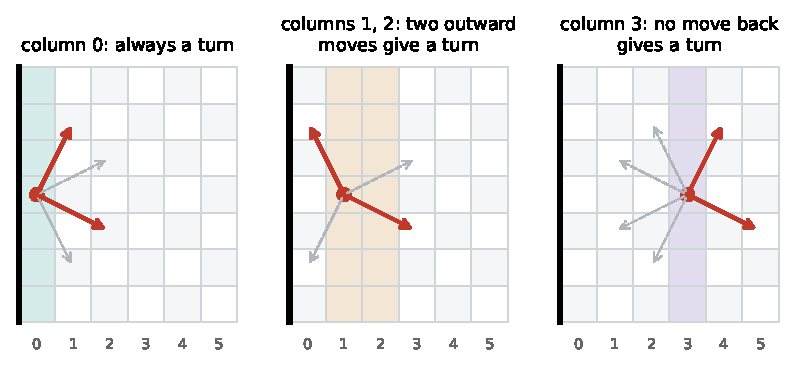
\includegraphics[width=\textwidth]{figures/lemma.pdf}
\caption{The three local facts in Lemma~\ref{lem:four}. Red arrows: the two moves of the cell. Dashed arrows: other moves of the same type. Left: a cell in column $0$ has only moves to the right. Middle: a cell in column $1$ with two \emph{outward} moves (to column $0$ or column $3$) turns, because the horizontal steps $-1$ and $+2$ do not cancel. Right: a cell in column $3$ with no move back to columns $1,2$ has two moves to the right, so it turns.}
\label{fig:lemma}
\end{figure}

\begin{theorem}\label{thm:64}
Every $2$-factor of the $n\times n$ knight graph, $n\ge8$, has at least $8n-64$ turns.
\end{theorem}

\begin{proof}
By symmetry, Lemma~\ref{lem:four} holds for the four columns or rows next to each of the four sides.
(A reflection of the board maps knight moves to knight moves and keeps opposite moves opposite.)
The sum of the four strip counts is at least $8n$.
For $n\ge 8$, opposite strips are disjoint.
Two adjacent strips meet in a $4\times4$ corner square.
So a cell is counted at most twice, and only the $64$ cells of the four corner squares can be counted twice.
Hence $T\ge 8n-64$.
\end{proof}

\begin{remark}
The coefficient $2$ in Lemma~\ref{lem:four} is sharp, also in a long strip.
Take the half-plane $x\ge0$, and give each cell in column $0$ the moves $(2,-1)$ and $(1,-2)$, each cell in column $1$ the moves $(2,-1)$ and $(-1,2)$, and every other cell the opposite moves $(2,-1)$ and $(-2,1)$.
These choices are symmetric, every cell has two neighbours, and only columns $0$ and $1$ turn.
The left side of our tours in Section~\ref{sec:upper} uses exactly this pattern.
\end{remark}

\subsection{The corner certificate: from 64 to 28}\label{sec:corner}

The proof of Theorem~\ref{thm:64} loses up to $16$ turns in each corner.
We now show that the true loss is at most $7$ per corner.
For this we write the proof of Lemma~\ref{lem:four} as a sum of local bounds.

For a cell $v$ at distance $i$ from one side of the board, define $L_i(v)$ from the two neighbours of $v$ in $F$, with distances measured from the same side:
\begin{align*}
L_0(v) &= 1,\\
L_1(v) = L_2(v) &= (\text{number of neighbours at distance $0$ or $3$}) - 1,\\
L_3(v) &= 1 - (\text{number of neighbours at distance $1$ or $2$}),\\
L_i(v) &= 0 \quad\text{for } i\ge4.
\end{align*}
The proof of Lemma~\ref{lem:four} shows two facts.
First, $t(v)\ge L_i(v)$ for every cell.
Second, the sum of $L_i$ over one strip is \emph{exactly} $2n$: the three sums are $n$, $(2n+B)-2n=B$, and $n-B$.

Let $L(v)$ be the sum of the four side contributions at $v$.
Then $\sum_v L(v)=8n$, and therefore
\[ T-8n \;=\; \sum_v \bigl(t(v)-L(v)\bigr). \]
For $n\ge8$, a cell outside the four corner squares has at most one nonzero side contribution, so $t(v)-L(v)\ge 0$ there.
It remains to bound the sum over each corner square from below.

Fix a corner.
Use coordinates $0\le x,y\le 3$, measured inward from its two sides, and write $L_x$ and $L_y$ for the contributions of the side at distance $x$ and of the side at distance $y$.
Put $r(v)=t(v)-L_x(v)-L_y(v)$.

\begin{lemma}[corner lemma]\label{lem:corner}
In every corner, $\sum_{v} r(v)\ge -7$, where the sum is over the $16$ cells of the corner square.
\end{lemma}

\begin{proof}
Define the numbers $\alpha(v)$ by Table~\ref{tab:alpha}, and the numbers $\beta(e)$ on nine edges $e$ inside the corner by Table~\ref{tab:beta}.
Let $\beta(e)=0$ for every other edge.
Each edge $e$ in Table~\ref{tab:beta} is written with its endpoints in lexicographic order, $e=(u,w)$ with $u<w$.
For a cell $v$, let
\[ D(v) \;=\; \sum_{e\ni v} \pm\beta(e), \]
where the sum is over the two edges of $F$ at $v$, with sign $+$ if $v$ is the first endpoint of $e$ and $-$ if it is the second.
We claim the local inequality
\begin{equation}\label{eq:cert}
r(v)\;\ge\;\alpha(v)+D(v)\qquad\text{for every cell $v$ of the corner and every choice of its two edges.}
\end{equation}
Inequality~\eqref{eq:cert} depends only on $v$ and on its two moves.
The moves must stay at nonnegative coordinates; for $n\ge8$ the board size gives no other restriction near a corner.
So~\eqref{eq:cert} is a finite statement with $209$ cases (cell, unordered pair of distinct moves).
All $209$ cases hold (finite check C1 in Appendix~\ref{app:repro}).
Every cell has a case with equality.

Now sum~\eqref{eq:cert} over the $16$ cells.
Every edge with $\beta(e)\ne0$ has both endpoints in the corner square.
If such an edge is in $F$, it contributes $+\beta(e)$ at one endpoint and $-\beta(e)$ at the other.
So $\sum_v D(v)=0$, and $\sum_v r(v)\ge\sum_v\alpha(v)=-7$.
\end{proof}

\begin{table}[t]
\centering
\begin{minipage}[t]{0.38\textwidth}
\centering
\begin{tabular}{c|rrrr}
 & $x=0$ & $1$ & $2$ & $3$\\\midrule
$y=0$ & $-1$ & $0$ & $0$ & $-1$\\
$y=1$ & $0$ & $1$ & $0$ & $-1$\\
$y=2$ & $0$ & $0$ & $0$ & $-1$\\
$y=3$ & $-1$ & $-1$ & $-1$ & $-1$
\end{tabular}
\caption{The numbers $\alpha(x,y)$. Their sum is $-7$.}
\label{tab:alpha}
\end{minipage}\hfill
\begin{minipage}[t]{0.55\textwidth}
\centering
\begin{tabular}{lr@{\qquad}lr}
\toprule
edge & $\beta$ & edge & $\beta$\\\midrule
$(0,1)$--$(1,3)$ & $-1$ & $(1,2)$--$(3,3)$ & $-1$\\
$(0,2)$--$(2,3)$ & $-1$ & $(2,0)$--$(3,2)$ & $-1$\\
$(0,3)$--$(1,1)$ & $+1$ & $(2,1)$--$(3,3)$ & $-1$\\
$(1,0)$--$(3,1)$ & $-1$ & $(2,2)$--$(3,0)$ & $-1$\\
$(1,1)$--$(3,0)$ & $-1$ & & \\\bottomrule
\end{tabular}
\caption{The nine edges with $\beta\ne0$, in corner coordinates $(x,y)$.}
\label{tab:beta}
\end{minipage}
\end{table}

\begin{proof}[Proof of Theorem~\ref{thm:main}(a)]
Sum the corner lemma over the four corners and use $t(v)-L(v)\ge0$ elsewhere:
$T-8n=\sum_v(t(v)-L(v))\ge 4\cdot(-7)=-28$.
\end{proof}

\begin{remark}
The corner lemma is sharp as a local statement.
There is a choice of moves for the $16$ corner cells, with edges that leave the corner left free, that has $\sum r(v)=-7$, with consistent internal edges and no cycle inside the corner (finite check C2).
So this method cannot give a constant better than $28$.
This does not show that $28$ is the best constant for tours.
The same proof gives at least $4(w+h)-28$ turns for a $w\times h$ board with $w,h\ge8$.
\end{remark}

\subsection{Formal verification}\label{sec:lean}

Theorem~\ref{thm:64} is verified in Lean~4 with Mathlib (project \texttt{ktlean}, Lean version 4.35.0-rc3).
The statement is
\begin{verbatim}
theorem KT.ClosedTour.eight_mul_sub_64_le_numTurns (T : ClosedTour n)
    (hn : 8 <= n) : 8 * n - 64 <= T.numTurns
\end{verbatim}
In the formal definitions, a \texttt{ClosedTour n} is a bijection from positions $\{0,\dots,n^2-1\}$ to cells, such that cyclically consecutive positions are a knight move apart.
\texttt{numTurns} counts the positions $i$ where the cells at positions $i-1,i,i+1$ are not collinear (collinear means a zero cross product), which is Definition~1 of~\cite{bjmow}.
\texttt{\#print axioms} reports only \texttt{propext}, \texttt{Classical.choice} and \texttt{Quot.sound}.
The project also proves the same bound for every $2$-factor (\texttt{KT.TwoFactor.eight\_mul\_le\_numTurns\_add}) and contains an explicit $8\times8$ tour, so the hypothesis is not empty.
The corner lemma (constant $28$) is not formalized.

\section{Upper bound}\label{sec:upper}

We describe one closed tour $\tau_n$ for each even $n\ge48$ (the family \emph{TT16}).
We give each cell its two moves.
The moves of a cell are written as two digits $jk$, with move codes
\begin{align*}
&0:(1,2),\quad &&1:(2,1),\quad &&2:(2,-1),\quad &&3:(1,-2),\\
&4:(-1,-2),\quad &&5:(-2,-1),\quad &&6:(-2,1),\quad &&7:(-1,2).
\end{align*}
Codes $k$ and $k+4$ (modulo $8$) are opposite, so a cell is straight exactly when its two digits differ by $4$.

\subsection{The construction}

\paragraph{Interior.}
Every cell not listed below has the code $26$: the moves $(2,-1)$ and $(-2,1)$.
These cells are straight.
They lie on the lines $c=x+2y$, which run from the upper left to the lower right with slope $-1/2$.

\paragraph{Bottom side.}
The four rows $y=0,1,2,3$ use the following template of period $8$.
Cell $(x,y)$ uses column $k=x\bmod 8$ of row $y$:
\begin{center}\ttfamily
\begin{tabular}{l|cccccccc}
\normalfont $y\backslash k$ & 0&1&2&3&4&5&6&7\\\midrule
3 & 26&26&26&26&26&26&26&26\\
2 & 36&26&26&46&26&46&36&26\\
1 & 25&26&25&26&26&25&26&25\\
0 & 16&67&06&16&06&16&16&67
\end{tabular}
\end{center}

\paragraph{Top side.}
The top side is the bottom side turned by $180^\circ$, with a shift.
Cell $(x,n-1-y)$, $y\le3$, uses the template entry of row $y$ and column $k=(1-x)\bmod 8$, with both moves negated.

\paragraph{Left and right sides.}
On the left, every cell in column $0$ has the moves $(2,-1),(1,-2)$ (code $23$), and every cell in column $1$ has the moves $(2,-1),(-1,2)$ (code $27$).
On the right, every cell in column $n-1$ has the moves $(-1,-2),(-2,1)$ (code $46$), and every cell in column $n-2$ has the moves $(-2,1),(1,2)$ (code $06$).

\paragraph{Corners.}
Each of the four $6\times6$ corner squares has fixed moves that depend only on $n\bmod 8$.
Appendix~\ref{app:corners} lists them: $4$ residues times $4$ corners.
The corner moves override all rules above.

\medskip
Figures~\ref{fig:bottom} and~\ref{fig:left} show parts of $\tau_{48}$, and Figure~\ref{fig:tour} shows all of it.
On the bottom side, each cell of row $0$ turns, about half the cells of rows $1$ and $2$ turn, and row $3$ is straight.
On the left side, columns $0$ and $1$ turn and everything else is straight.

\begin{figure}[t]
\centering
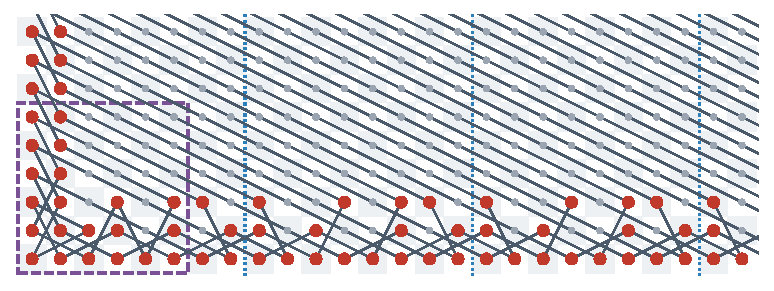
\includegraphics[width=\textwidth]{figures/band_bottom.pdf}
\caption{Bottom-left part of $\tau_{48}$, columns $0$--$25$, rows $0$--$8$. Red: turns. Grey: straight cells. Dashed square: the $6\times6$ corner square. Dotted lines: the period boundaries of the bottom template (period $8$). Each period has $16$ turns.}
\label{fig:bottom}
\end{figure}

\begin{figure}[t]
\centering
\begin{minipage}[b]{0.3\textwidth}\centering
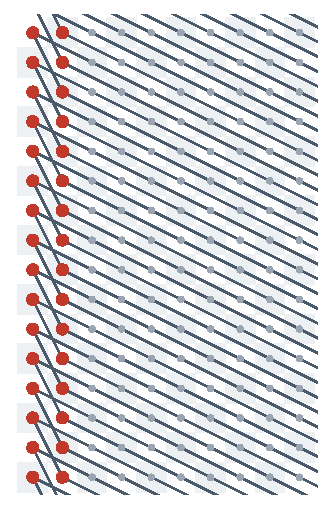
\includegraphics[height=7.5cm]{figures/band_left.pdf}
\caption{Left side of $\tau_{48}$, columns $0$--$9$, rows $14$--$29$. Two turns per row.}
\label{fig:left}
\end{minipage}\hfill
\begin{minipage}[b]{0.66\textwidth}\centering
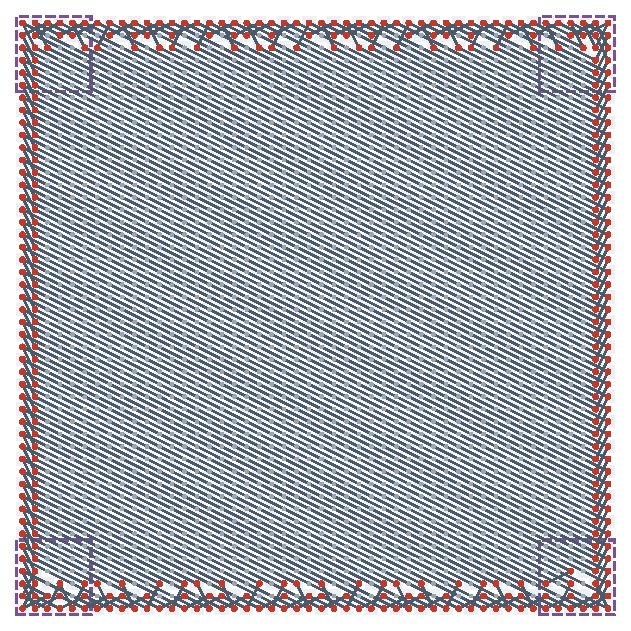
\includegraphics[width=\textwidth]{figures/tour48.pdf}
\caption{The tour $\tau_{48}$, with $8\cdot48-14=370$ turns (red).}
\label{fig:tour}
\end{minipage}
\end{figure}

\subsection{The turn count}

\begin{lemma}\label{lem:count}
For every even $n\ge48$, $\tau_n$ has exactly $8n-14$ turns.
\end{lemma}

\begin{proof}
A cell is a turn or not according to its own two moves only.
So we count cell by cell.

\emph{Interior cells} are straight.

\emph{Bottom and top.}
Let $c_k$ be the number of turns in column $k$ of the bottom template.
Row $0$ turns everywhere, row $3$ nowhere, row $1$ at $k\in\{0,2,5,7\}$ and row $2$ at $k\in\{0,3,5,6\}$.
So $(c_0,\dots,c_7)=(3,1,2,2,1,3,2,2)$, and $c_k+c_{(1-k)\bmod 8}=4$ for every $k$.
Column $x$ of the board uses template column $x\bmod 8$ at the bottom and $(1-x)\bmod 8$ at the top.
So every column $x$ with $6\le x\le n-7$ has exactly $4$ turns in its bottom and top rows.

\emph{Left and right.}
Every row $y$ with $6\le y\le n-7$ has exactly $2$ turns on the left and $2$ on the right.

\emph{Corners.}
For each residue of $n$ modulo $8$, the four corner squares of Appendix~\ref{app:corners} contain $82$ turns in total.

Adding up, $T(\tau_n)=82+4(n-12)+4(n-12)=8n-14$.
\end{proof}

The count is the same for every residue, but the corner squares differ.
The residue matters only for the connectivity, which we show next.

\subsection{One cycle for every \texorpdfstring{$n$}{n}}\label{sec:onecycle}

The rules above give every cell two moves.
A finite check (C3) confirms, for each even $n$ from $48$ to $102$, that the moves are symmetric (if $u$ uses a move to $w$, then $w$ uses the opposite move to $u$) and that the resulting $2$-factor is a single cycle through all $n^2$ cells.
We now show that the step from $n$ to $n+8$ keeps a single cycle, for $n\ge96$.
With the bases $n=96,98,100,102$, this covers every even $n\ge 48$.

\paragraph{Line labels.}
Give each cell the label $c=x+2y$.
Interior edges keep $c$ fixed, and every knight move changes $c$ by at most $5$.
For each $c$, each maximal run of interior cells with label $c$ is a straight path.
We \emph{suppress} the inner cells of these paths (replace each path by one edge).
This keeps the number of cycles.

Away from the corners, the two ends of an interior line lie in two side bands, as follows:
\begin{center}
\begin{tabular}{ll}
\toprule
range of $c$ & bands at the two ends of line $c$\\\midrule
$24<c<n-24$ & bottom and left\\
$n+24<c<2n-24$ & left and right\\
$2n+24<c<3n-24$ & right and top\\\bottomrule
\end{tabular}
\end{center}
The corner squares have label ranges $[0,15]$, $[n-6,n+9]$, $[2n-12,2n+3]$ and $[3n-18,3n-3]$.
The margin $24$ keeps the three ranges away from the corners and from the places where a line changes its band pair.

\paragraph{Blocks.}
A \emph{block} is the set of (non-suppressed) cells with labels in $[a,a+8)$, for a cut $a$ such that $[a,a+8)$ lies in one of the three ranges.
No edge jumps over a block, because $8>5$.
A \emph{port} is an edge with one end in the block and one end outside.
Inside one range, the side templates have period $8$ in $c$: the bottom and top templates have period $8$ in $x$, the left and right templates have period $4$ in $y$, and $c$ changes by $8$ under these shifts.
So the block at cut $a$ and the block at cut $a+8$ are translates of each other, with the same ports.
We number the ports of a cut by sorting their descriptions (band, the distances of both ends from the side, and the label offsets of both ends from the cut).
Write $L_i$ and $R_i$ for port $i$ at the left cut $a$ and at the right cut $a+8$.

Inside a block, the cells form paths whose ends are ports.
The \emph{complete matching} $M$ of a block pairs the two ends of each path.
It includes paths that return to the same cut.
Finite check C4 traces the blocks of $\tau_{96},\dots,\tau_{102}$ at the cuts $a=35$, $a=$ the first multiple of $8$ that is at least $n+32$, and $a=2n+32$.
It confirms that every cell of the block lies on one of these paths (so there is no cycle inside the block), and that the matchings are:
\begin{center}
\begin{tabular}{ll}
\toprule
range & complete matching $M$\\\midrule
bottom--left & $L_0$--$R_3$, $L_1$--$L_3$, $L_2$--$R_2$, $R_0$--$R_1$\\
left--right & $L_0$--$R_0$, $L_1$--$R_1$, $L_2$--$R_2$, $L_3$--$R_3$\\
right--top & $L_0$--$L_2$, $L_1$--$R_3$, $L_3$--$L_5$, $L_4$--$R_0$, $R_1$--$R_5$, $R_2$--$R_4$\\\bottomrule
\end{tabular}
\end{center}

\paragraph{Two copies act like one.}
Glue two copies of a block: the right port $R_i$ of the first copy is the left port $L_i$ of the second copy.
For each of the three matchings, the glued system pairs its outer ports exactly as $M$ does, and the gluing closes no cycle.
We write this as $M^2=M$.
For example, in the bottom--left block, the path from $L_0$ of the first copy reaches $R_3$, continues in the second copy through the return path $L_3$--$L_1$, comes back to the first copy at $R_1$, follows $R_1$--$R_0$, and enters the second copy at $L_0$, where it continues to $R_3$.
So the glued system again pairs the outer $L_0$ with the outer $R_3$.
The other cases are similar and are part of check C4.

\paragraph{The step from $n$ to $n+8$.}
Choose one block in each of the three ranges.
Replace each of them by two copies, so that the labels after the first, second and third insertion shift by $8$, $16$ and $24$.
Move each cell of a side band by the vector below, where $r\in\{0,1,2,3\}$ is the number of insertions before its label:
\begin{center}
\begin{tabular}{lcccc}
\toprule
band & bottom & left & right & top\\\midrule
shift $(\Delta x,\Delta y)$ & $(8r,0)$ & $(0,4r)$ & $(8,4(r-1))$ & $(8(r-2),8)$\\\bottomrule
\end{tabular}
\end{center}
Each shift changes $c$ by $8r$ and keeps the distance to the side.
The bottom and top shifts are multiples of $8$ in $x$, and the left and right shifts are multiples of $4$ in $y$, so every template phase is kept.
The four corners move by $(0,0)$, $(8,0)$, $(0,8)$ and $(8,8)$, which is where the corners of the $(n+8)\times(n+8)$ board are.
The corner squares of $n$ and $n+8$ are the same, because they depend only on $n\bmod8$.
Each interior line still joins the same two ports; only its length changes.
So the result is exactly the reduced graph of $\tau_{n+8}$.
(Check C4 also compares the actual $16$-label block of $\tau_{n+8}$ with the glued two copies, and the internal audit compared the whole exterior graph; see Appendix~\ref{app:repro}.)

\paragraph{Conclusion.}
By $M^2=M$, the inserted material connects the outside ports exactly as the old block did, and it contains no separate cycle.
Every other part of the graph is unchanged up to translation and the length of straight paths.
So if $\tau_n$ is one cycle, then $\tau_{n+8}$ is one cycle.
With the bases $96,\dots,102$, this proves that $\tau_n$ is a closed tour for every even $n\ge96$; check C3 covers $48\le n\le 94$ directly.
Together with Lemma~\ref{lem:count}, this proves Theorem~\ref{thm:main}(b).

\section{Remarks and open questions}

\begin{enumerate}
\item The gap between the bounds is $14$.
The lower-bound method cannot do better than $8n-28$ (the corner lemma is sharp locally), so a better lower bound needs larger corner regions or a new argument.
On the upper side, our corner squares were found by a computer search over the $6\times6$ corner squares, with the side templates fixed. This does not show that $8n-14$ is best possible.
\item The construction uses exactly the minimum average rate of $2$ turns per row or column at each side (Lemma~\ref{lem:four}).
So, up to the constant, the turns of an optimal tour are where the lower bound puts them.
\item We do not consider open tours or non-square boards here.
\todo{Nil: decide whether to mention crossings (the same project has separate crossing results) or keep this note about turns only.}
\end{enumerate}

\appendix

\section{Reproducibility and audit status}\label{app:repro}

All checks use only the Python standard library and the data files below, unless stated otherwise.
No check imports a solver.
Paths are relative to the project repository. \todo{public repository location}

\begin{description}
\item[C1 (corner lemma, 209 cases).] Run \texttt{python3} \path{writeup/turns/check_corner.py}. It checks inequality~\eqref{eq:cert} with the numbers exactly as printed in Tables~\ref{tab:alpha} and~\ref{tab:beta}. A separate earlier checker, \path{w-turnstheory/check_corner_certificate.py}, checks the same certificate from its own data and also on generated tours. The script \path{w-turnstheory/check_proof.py} checks the $77$ one-side cases of Lemma~\ref{lem:four}.
\item[C2 (sharpness of the corner lemma).] \path{w-turnstheory/check_corner_certificate.py}, with the data in \path{w-turnstheory/corner_witness.txt}.
\item[C3 (the tours $\tau_n$, $48\le n\le102$).] Run \path{.venv/bin/python} \path{writeup/turns/figures/tt16.py}. It builds $\tau_n$ from the corner files \path{w-integrator/corners/TT16_res*.json}, checks that it is a closed tour, checks $T=8n-14$, counts the $82$ corner turns, and writes the figures and the tables of Appendix~\ref{app:corners}. Matplotlib is used only for the figures.
\item[C4 (block insertion).] Run \texttt{python3} \path{w-turnstheory/check_upper_proofs.py}. It rebuilds the tours, traces the blocks, and checks the complete matchings, $M^2=M$ without closed components, the equality of the actual longer block with two glued copies, and the turn increment $64$ per step. It writes the ports and matchings to \path{upper_proof_checks.json}.
\item[Lean.] In \path{ktlean/}, run \texttt{lake build}, and then \texttt{lake env lean Axioms.lean} to print the axioms.
\end{description}

\paragraph{Audit status (2026-10-02).}
Theorem~\ref{thm:64}, Lemma~\ref{lem:corner} and the construction with its block-insertion proof were each checked by an independent internal reviewer with separately written code.
That review rebuilt $\tau_n$ for every even $n$ from $48$ to $134$ and for $n=312,\dots,318$, and compared the full exterior graph after insertion for the four residues.
The Lean build and the axiom report were rerun by a second person.
The text of this note, the checker \texttt{check\_corner.py} and the script \texttt{tt16.py} were independently reviewed on 2026-10-02 (hand count, both certificates, the theorem statements); the corrections from that review are applied.
\todo{external review}

\section{The corner squares}\label{app:corners}

Each table gives the move codes of one $6\times6$ corner square, with the top row first and the leftmost column first.
TL is the square $0\le x\le5$, $n-6\le y\le n-1$; TR is $n-6\le x\le n-1$, $n-6\le y\le n-1$; BL is $0\le x,y\le5$; BR is $n-6\le x\le n-1$, $0\le y\le5$.

\paragraph{Residue $n\equiv 0\pmod 8$.}
\begin{center}\scriptsize\ttfamily
\begin{tabular}[t]{@{}c@{\,}c@{\,}c@{\,}c@{\,}c@{\,}c@{}}\multicolumn{6}{c}{\normalfont\scriptsize TL}\\
23 & 23 & 25 & 25 & 23 & 25\\
13 & 12 & 26 & 16 & 16 & 26\\
23 & 27 & 27 & 26 & 26 & 27\\
23 & 27 & 26 & 26 & 26 & 26\\
23 & 27 & 26 & 26 & 26 & 26\\
23 & 27 & 26 & 26 & 26 & 26\end{tabular}\qquad
\begin{tabular}[t]{@{}c@{\,}c@{\,}c@{\,}c@{\,}c@{\,}c@{}}\multicolumn{6}{c}{\normalfont\scriptsize TR}\\
23 & 25 & 23 & 23 & 35 & 45\\
26 & 26 & 16 & 16 & 36 & 46\\
26 & 27 & 26 & 67 & 07 & 47\\
26 & 26 & 26 & 26 & 06 & 47\\
26 & 26 & 26 & 26 & 06 & 46\\
26 & 26 & 26 & 26 & 06 & 46\end{tabular}\qquad
\begin{tabular}[t]{@{}c@{\,}c@{\,}c@{\,}c@{\,}c@{\,}c@{}}\multicolumn{6}{c}{\normalfont\scriptsize BL}\\
23 & 27 & 26 & 26 & 26 & 26\\
23 & 27 & 26 & 26 & 26 & 26\\
23 & 47 & 26 & 26 & 26 & 26\\
23 & 47 & 26 & 34 & 26 & 46\\
02 & 27 & 56 & 25 & 26 & 25\\
01 & 17 & 06 & 16 & 07 & 16\end{tabular}\qquad
\begin{tabular}[t]{@{}c@{\,}c@{\,}c@{\,}c@{\,}c@{\,}c@{}}\multicolumn{6}{c}{\normalfont\scriptsize BR}\\
26 & 26 & 26 & 26 & 06 & 46\\
26 & 26 & 26 & 26 & 06 & 46\\
26 & 26 & 56 & 26 & 06 & 46\\
16 & 26 & 46 & 26 & 03 & 46\\
25 & 26 & 25 & 26 & 05 & 56\\
16 & 06 & 16 & 16 & 06 & 67\end{tabular}
\end{center}

\paragraph{Residue $n\equiv 2\pmod 8$.}
\begin{center}\scriptsize\ttfamily
\begin{tabular}[t]{@{}c@{\,}c@{\,}c@{\,}c@{\,}c@{\,}c@{}}\multicolumn{6}{c}{\normalfont\scriptsize TL}\\
23 & 23 & 25 & 25 & 23 & 25\\
13 & 12 & 26 & 16 & 16 & 26\\
23 & 27 & 27 & 26 & 26 & 27\\
23 & 27 & 26 & 26 & 26 & 26\\
23 & 27 & 26 & 26 & 26 & 26\\
23 & 27 & 26 & 26 & 26 & 26\end{tabular}\qquad
\begin{tabular}[t]{@{}c@{\,}c@{\,}c@{\,}c@{\,}c@{\,}c@{}}\multicolumn{6}{c}{\normalfont\scriptsize TR}\\
25 & 24 & 23 & 23 & 35 & 45\\
26 & 26 & 16 & 16 & 36 & 46\\
02 & 26 & 26 & 67 & 07 & 47\\
26 & 26 & 26 & 26 & 06 & 47\\
26 & 26 & 26 & 26 & 06 & 46\\
26 & 26 & 26 & 26 & 06 & 46\end{tabular}\qquad
\begin{tabular}[t]{@{}c@{\,}c@{\,}c@{\,}c@{\,}c@{\,}c@{}}\multicolumn{6}{c}{\normalfont\scriptsize BL}\\
23 & 27 & 26 & 26 & 26 & 26\\
23 & 27 & 26 & 26 & 26 & 26\\
23 & 47 & 26 & 26 & 26 & 26\\
23 & 47 & 26 & 34 & 26 & 46\\
02 & 27 & 56 & 25 & 26 & 25\\
01 & 17 & 06 & 16 & 07 & 16\end{tabular}\qquad
\begin{tabular}[t]{@{}c@{\,}c@{\,}c@{\,}c@{\,}c@{\,}c@{}}\multicolumn{6}{c}{\normalfont\scriptsize BR}\\
26 & 26 & 26 & 26 & 06 & 46\\
26 & 26 & 26 & 26 & 06 & 46\\
26 & 26 & 36 & 26 & 06 & 46\\
26 & 46 & 46 & 26 & 03 & 46\\
26 & 25 & 26 & 27 & 05 & 56\\
06 & 06 & 16 & 16 & 06 & 67\end{tabular}
\end{center}

\paragraph{Residue $n\equiv 4\pmod 8$.}
\begin{center}\scriptsize\ttfamily
\begin{tabular}[t]{@{}c@{\,}c@{\,}c@{\,}c@{\,}c@{\,}c@{}}\multicolumn{6}{c}{\normalfont\scriptsize TL}\\
23 & 23 & 25 & 25 & 23 & 25\\
13 & 12 & 26 & 16 & 16 & 26\\
23 & 27 & 27 & 26 & 26 & 27\\
23 & 27 & 26 & 26 & 26 & 26\\
23 & 27 & 26 & 26 & 26 & 26\\
23 & 27 & 26 & 26 & 26 & 26\end{tabular}\qquad
\begin{tabular}[t]{@{}c@{\,}c@{\,}c@{\,}c@{\,}c@{\,}c@{}}\multicolumn{6}{c}{\normalfont\scriptsize TR}\\
25 & 24 & 23 & 25 & 34 & 45\\
26 & 16 & 26 & 16 & 36 & 46\\
02 & 26 & 26 & 07 & 06 & 47\\
26 & 26 & 26 & 26 & 06 & 47\\
26 & 26 & 26 & 26 & 06 & 46\\
26 & 26 & 26 & 26 & 06 & 46\end{tabular}\qquad
\begin{tabular}[t]{@{}c@{\,}c@{\,}c@{\,}c@{\,}c@{\,}c@{}}\multicolumn{6}{c}{\normalfont\scriptsize BL}\\
23 & 27 & 26 & 26 & 26 & 26\\
23 & 27 & 26 & 26 & 26 & 26\\
23 & 47 & 26 & 26 & 26 & 26\\
23 & 47 & 26 & 34 & 26 & 46\\
02 & 27 & 56 & 25 & 26 & 25\\
01 & 17 & 06 & 16 & 07 & 16\end{tabular}\qquad
\begin{tabular}[t]{@{}c@{\,}c@{\,}c@{\,}c@{\,}c@{\,}c@{}}\multicolumn{6}{c}{\normalfont\scriptsize BR}\\
26 & 26 & 26 & 26 & 06 & 46\\
26 & 26 & 26 & 26 & 06 & 46\\
26 & 26 & 36 & 26 & 06 & 46\\
26 & 46 & 46 & 26 & 03 & 46\\
26 & 25 & 26 & 27 & 05 & 56\\
06 & 06 & 16 & 16 & 06 & 67\end{tabular}
\end{center}

\paragraph{Residue $n\equiv 6\pmod 8$.}
\begin{center}\scriptsize\ttfamily
\begin{tabular}[t]{@{}c@{\,}c@{\,}c@{\,}c@{\,}c@{\,}c@{}}\multicolumn{6}{c}{\normalfont\scriptsize TL}\\
23 & 23 & 25 & 25 & 23 & 25\\
13 & 12 & 26 & 16 & 16 & 26\\
23 & 27 & 27 & 26 & 26 & 27\\
23 & 27 & 26 & 26 & 26 & 26\\
23 & 27 & 26 & 26 & 26 & 26\\
23 & 27 & 26 & 26 & 26 & 26\end{tabular}\qquad
\begin{tabular}[t]{@{}c@{\,}c@{\,}c@{\,}c@{\,}c@{\,}c@{}}\multicolumn{6}{c}{\normalfont\scriptsize TR}\\
23 & 25 & 24 & 23 & 35 & 45\\
26 & 26 & 16 & 16 & 36 & 46\\
26 & 07 & 26 & 26 & 07 & 47\\
26 & 26 & 26 & 23 & 06 & 67\\
26 & 26 & 26 & 26 & 06 & 46\\
26 & 26 & 26 & 26 & 67 & 46\end{tabular}\qquad
\begin{tabular}[t]{@{}c@{\,}c@{\,}c@{\,}c@{\,}c@{\,}c@{}}\multicolumn{6}{c}{\normalfont\scriptsize BL}\\
23 & 27 & 26 & 26 & 26 & 26\\
23 & 27 & 26 & 26 & 26 & 26\\
23 & 47 & 26 & 26 & 26 & 26\\
23 & 47 & 26 & 34 & 26 & 46\\
02 & 27 & 56 & 25 & 26 & 25\\
01 & 17 & 06 & 16 & 07 & 16\end{tabular}\qquad
\begin{tabular}[t]{@{}c@{\,}c@{\,}c@{\,}c@{\,}c@{\,}c@{}}\multicolumn{6}{c}{\normalfont\scriptsize BR}\\
26 & 26 & 26 & 26 & 06 & 46\\
26 & 26 & 26 & 26 & 06 & 46\\
26 & 26 & 56 & 26 & 06 & 46\\
16 & 26 & 46 & 26 & 03 & 46\\
25 & 26 & 25 & 26 & 05 & 56\\
16 & 06 & 16 & 16 & 06 & 67\end{tabular}
\end{center}


\section*{Acknowledgements}
\todo{acknowledgements}

\begin{thebibliography}{9}
\bibitem{bjmow} J.~J.~Besa, T.~Johnson, N.~Mamano, M.~C.~Osegueda, P.~Williams.
\newblock Taming the knight's tour: minimizing turns and crossings.
\newblock arXiv:1904.02824. \todo{journal version and year}
\end{thebibliography}

\end{document}
